%%
%% Copyright 2024 OXFORD UNIVERSITY PRESS
%%
%% This file is part of the 'mam-authoring-template Bundle'.
%% ---------------------------------------------
%%
%% It may be distributed under the conditions of the LaTeX Project Public
%% License, either version 1.2 of this license or (at your option) any
%% later version.  The latest version of this license is in
%%    http://www.latex-project.org/lppl.txt
%% and version 1.2 or later is part of all distributions of LaTeX
%% version 1999/12/01 or later.
%%
%% The list of all files belonging to the 'mam-authoring-template Bundle' is
%% given in the file `manifest.txt'.
%%
%% Template article for Microscopy and Microanalysis' document class `mam-authoring-template'
%% with bibliographic references
%%

\documentclass[unnumsec,webpdf,modern,large]{mam-authoring-template}%
\usepackage{amsmath,amssymb}
\usepackage{upgreek}
% natbib is already loaded by the document class
\bibliographystyle{plainnat}

% Suppress underfull hbox warnings
\hbadness=10000

\newcommand{\myfixed}{{\,\textrm{fixed}}}
\newcommand{\set}[1]{\left\{ #1 \right\}}
\newcommand{\myhier}{\textrm{hier}}
\newcommand{\myall}{\textrm{all}}
\newcommand{\mypair}{\textrm{pair}}
\newcommand{\myvar}{\textrm{var}}
\newcommand{\mygen}{\textrm{gen}}
\newcommand{\mysubsets}{\textrm{subsets}}
\newcommand{\mysource}{\textrm{source}}
\newcommand{\mysink}{\textrm{sink}}
\newcommand{\mytmp}{\textrm{tmp}}


%\usepackage{showframe}
\usepackage{upgreek}

\graphicspath{{figs/}}

% line numbers
%\usepackage[mathlines, switch]{lineno}
%\usepackage[right]{lineno}

\theoremstyle{thmstyleone}%
\newtheorem{theorem}{Theorem}%  meant for continuous numbers
%%\newtheorem{theorem}{Theorem}[section]% meant for sectionwise numbers
%% optional argument [theorem] produces theorem numbering sequence instead of independent numbers for Proposition
\newtheorem{proposition}[theorem]{Proposition}%
%%\newtheorem{proposition}{Proposition}% to get separate numbers for theorem and proposition etc.
\theoremstyle{thmstyletwo}%
\newtheorem{example}{Example}%
\newtheorem{remark}{Remark}%
\theoremstyle{thmstylethree}%
\newtheorem{definition}{Definition}

\begin{document}

\journaltitle{bioR$\upchi$i$\upnu$}
%\DOI{DOI HERE}
\copyrightyear{2025}
\pubyear{2025}
%\access{Advance Access Publication Date: Day Month Year}
\appnotes{Original Article}

\firstpage{1}

%\subtitle{Subject Section}

\title[PoolParty]{PoolParty: painless design of complex oligonucleotide pools in Python}

\author[1]{Zhihan Liu}
\author[1,$\ast$]{Justin B. Kinney\ORCID{0000-0003-1897-3778}}

\authormark{Liu and Kinney}

\address[1]{\orgdiv{Simons Center for Quantitative Biology}, \orgname{Cold Spring Harbor Laboratory}, \orgaddress{\street{1 Bungtown Rd.}, \postcode{11724}, \state{New York}, \country{United States}}}

\corresp[$\ast$]{Corresponding author. \href{email:jkinney@cshl.edu}{jkinney@cshl.edu}}

\received{Date}{0}{Year}
\revised{Date}{0}{Year}
\accepted{Date}{0}{Year}

\abstract{\textbf{Summary}: The use of designed oligonucleotide pools is rapidly expanding thanks to massively parallel reporter assays (MPRAs), protein deep mutational scanning (DMS), and other multiplexed assays of variant effect (MAVEs). Designing these pools, however, remains tedious and error-prone due to the lack of purpose-built software. Here we introduce PoolParty, a Python package for declarative, composable oligonucleotide pool design. PoolParty represents each design operation as a Pool---a stateful sequence generator---and allows Pools to be combined using intuitive algebraic operators to form directed acyclic computation graphs. This architecture enables users to specify complex multi-region, multi-stage library designs in just a few lines of code, while automatically maintaining per-sequence provenance metadata (``design cards'') for reproducibility and downstream analysis. PoolParty includes 20 specialized Pool types for nucleotide and codon-level mutagenesis, motif insertion, deletion and insertion scans, context-preserving shuffling, and barcode generation. An interactive visualization tool allows users to inspect the computation graph, view region-specific transformations, and audit individual sequences. PoolParty thus transforms oligonucleotide pool design from ad hoc scripting into a structured, transparent, and reproducible process. \\
\textbf{Availability and implementation:} PoolParty can be installed using the pip package manager and is compatible with Python $\geq$ 3.10. Documentation is provided at http://poolparty.readthedocs.io; source code is available at http://github.com/jbkinney/poolparty.\\
\textbf{Contact:} jkinney@cshl.edu (J.B.K.)}


\maketitle

\section{Introduction}

Designed oligonucleotide pools have become essential tools in modern functional genomics. Massively parallel reporter assays (MPRAs) use synthetic oligo libraries to measure the regulatory activity of thousands of sequence variants in a single experiment \citep{Inoue2015cs}. Deep mutational scanning (DMS) systematically mutates protein-coding sequences to map fitness landscapes and identify functional residues \citep{Fowler2014gq}. More broadly, multiplexed assays of variant effect (MAVEs) encompass a growing family of high-throughput approaches that leverage designed oligo pools to probe sequence-function relationships at unprecedented scale \citep{Kinney2019jc}.

These applications require libraries that encode systematic perturbations---point mutations, insertions, deletions, motif substitutions, codon-level edits---often combined with positional constraints, reading-frame preservation, and unique molecular barcodes. As experimental designs grow more sophisticated, the complexity of library specification grows accordingly. A typical project might require scanning mutations across a regulatory element, inserting candidate motifs at multiple positions, applying codon-aware edits to an open reading frame, and appending unique barcodes---all within a single oligonucleotide pool.

Several categories of existing tools address parts of this problem. General-purpose sequence toolkits such as BioPython \citep{Cock2009df}, tangermeme \citep{Schreiber2025nd}, pydna \citep{Pereira2015wj}, and SeqPro \citep{Klie2023kg} provide low-level operations for slicing, mutating, and manipulating sequences. However, these tools lack any notion of a library as a structured object; users must hand-code loops, region segmentation, and all associated bookkeeping. Assay-specific template designers such as MPRAnator \citep{GeorgakopoulosSoares2017gb}, MPRA Design Tool \citep{Ghazi2018aa}, and VaLiAnT \citep{Barbon2022th} offer streamlined pipelines for particular experimental formats, but their rigid templates make it difficult to express non-standard designs with multiple regions or multi-stage transformations. Constraint and optimization frameworks like DnaChisel \citep{Zulkower2020jk} and CodonGenie \citep{Swainston2017rb} optimize individual sequences under synthesis or biological constraints but do not define or traverse large library design spaces. Saturation mutagenesis tools such as Mutation Maker \citep{Hiraga2021yg} focus on primer design for PCR-based approaches rather than complete synthetic oligopools.

A significant gap therefore remains: no existing framework provides a unified, extensible approach for declarative, provenance-aware specification of large heterogeneous oligonucleotide libraries. PoolParty addresses this gap by introducing a compositional architecture in which each design operation is represented as a Pool---a stateful sequence generator---and Pools compose algebraically into directed acyclic graphs (DAGs) that encode region-specific, multi-stage transformations (Fig.~1). This architecture shifts library design from imperative string manipulation to declarative generative specification, reducing user burden, minimizing procedural errors, and enabling transparent, reproducible workflows for high-throughput genomics.

\section{Methods}

\subsection{Pool abstractions and composition}

PoolParty's core abstraction is the Pool, a stateful generator that produces sequences on demand. Pools fall into two categories (Fig.~1A). Source Pools generate sequences from scratch: examples include literal strings, KmerPool (all k-mers), BarcodePool (random or enumerated barcodes), IUPACPool (sequences matching IUPAC ambiguity codes), and MotifPool (sequences drawn from a motif model). Modifier Pools transform sequences produced by an upstream Pool: examples include KMutationPool and RandomMutationPool for nucleotide-level mutagenesis, InsertionScanPool and DeletionScanPool for systematic indel libraries, ShufflePool for context-preserving randomization, and SubseqPool for extracting subsequences. A parallel set of ORF-aware modifier Pools (e.g., KMutationORFPool, InsertionScanORFPool, DeletionScanORFPool) operate at the codon level to preserve reading frames when mutating coding sequences.

Pools compose using three algebraic operators that mirror Python's string syntax. The concatenation operator (\texttt{+}) joins Pools end-to-end, the repeat operator (\texttt{*}) duplicates a Pool a specified number of times, and the slice operator (\texttt{[]}) extracts a contiguous subsequence. These operators return new composite Pool objects, allowing users to build arbitrarily complex designs through nested expressions. Internally, composite Pools form a directed acyclic computation graph (Fig.~1B), with source Pools at the leaves, modifier Pools as intermediate nodes, and the final composite Pool at the root.

\subsection{Sequence generation}

PoolParty employs lazy evaluation: sequences are generated only when explicitly requested via the \texttt{generate\_seqs()} method. Each Pool maintains an internal state that determines which sequence it produces for a given global index. When a composite Pool generates its $n$-th sequence, it uses mixed-radix decomposition to map the global index $n$ to local indices for each constituent Pool, then assembles the final sequence by concatenating or transforming the outputs of its children.

Critically, each Pool can operate in either sequential or random mode. In sequential mode, a Pool enumerates its state space exhaustively---useful for systematic scans or complete enumeration of small variant sets. In random mode, the Pool samples states stochastically using a reproducible pseudorandom number generator seeded by the global index---useful for barcodes, large mutation spaces, or stochastic sampling within otherwise deterministic designs. Because mode is set per-Pool, users can freely mix exhaustive enumeration and stochastic sampling across different regions and stages of a single library (Fig.~1C).

\subsection{Design cards and visualization}

To support reproducibility and downstream analysis, PoolParty automatically generates per-sequence metadata called design cards (Fig.~1D). Each design card records which transformations fired at which positions, with which internal states, for a given sequence. For example, a design card might indicate that sequence 42 has mutations at positions 3 and 13 (G$\rightarrow$C and G$\rightarrow$T), a motif inserted starting at position 0, and the motif sequence AAGTC. Design cards are returned as structured data alongside the generated sequences, enabling users to filter, group, and analyze library members by their generative provenance.

PoolParty also provides an interactive visualization tool (Fig.~1E) that displays three synchronized views: a Linear Sequence View showing the stacked regional architecture of each sequence, a Graph View depicting the DAG of Pool nodes, and a Node Details panel summarizing the selected Pool's parameters, state space, and sample sequences. Users can step through sequences, inspect which Pool produced each region, and identify design errors before synthesis.

\subsection{Implementation and extensibility}

PoolParty is implemented in pure Python and requires Python 3.10 or later. The package has minimal dependencies (NumPy for numerical operations) and is distributed under an open-source license via PyPI. Comprehensive documentation, tutorials, and example notebooks are available at the project website.

The architecture is designed for extensibility. New Pool types can be created by subclassing the base Pool class and implementing a small number of methods (state space size, sequence generation, metadata extraction). Custom Pools automatically inherit support for algebraic composition, global-state indexing, design card generation, and visualization, allowing researchers to extend PoolParty with domain-specific operations without reimplementing core infrastructure.

\begin{figure*}[t]
\centering
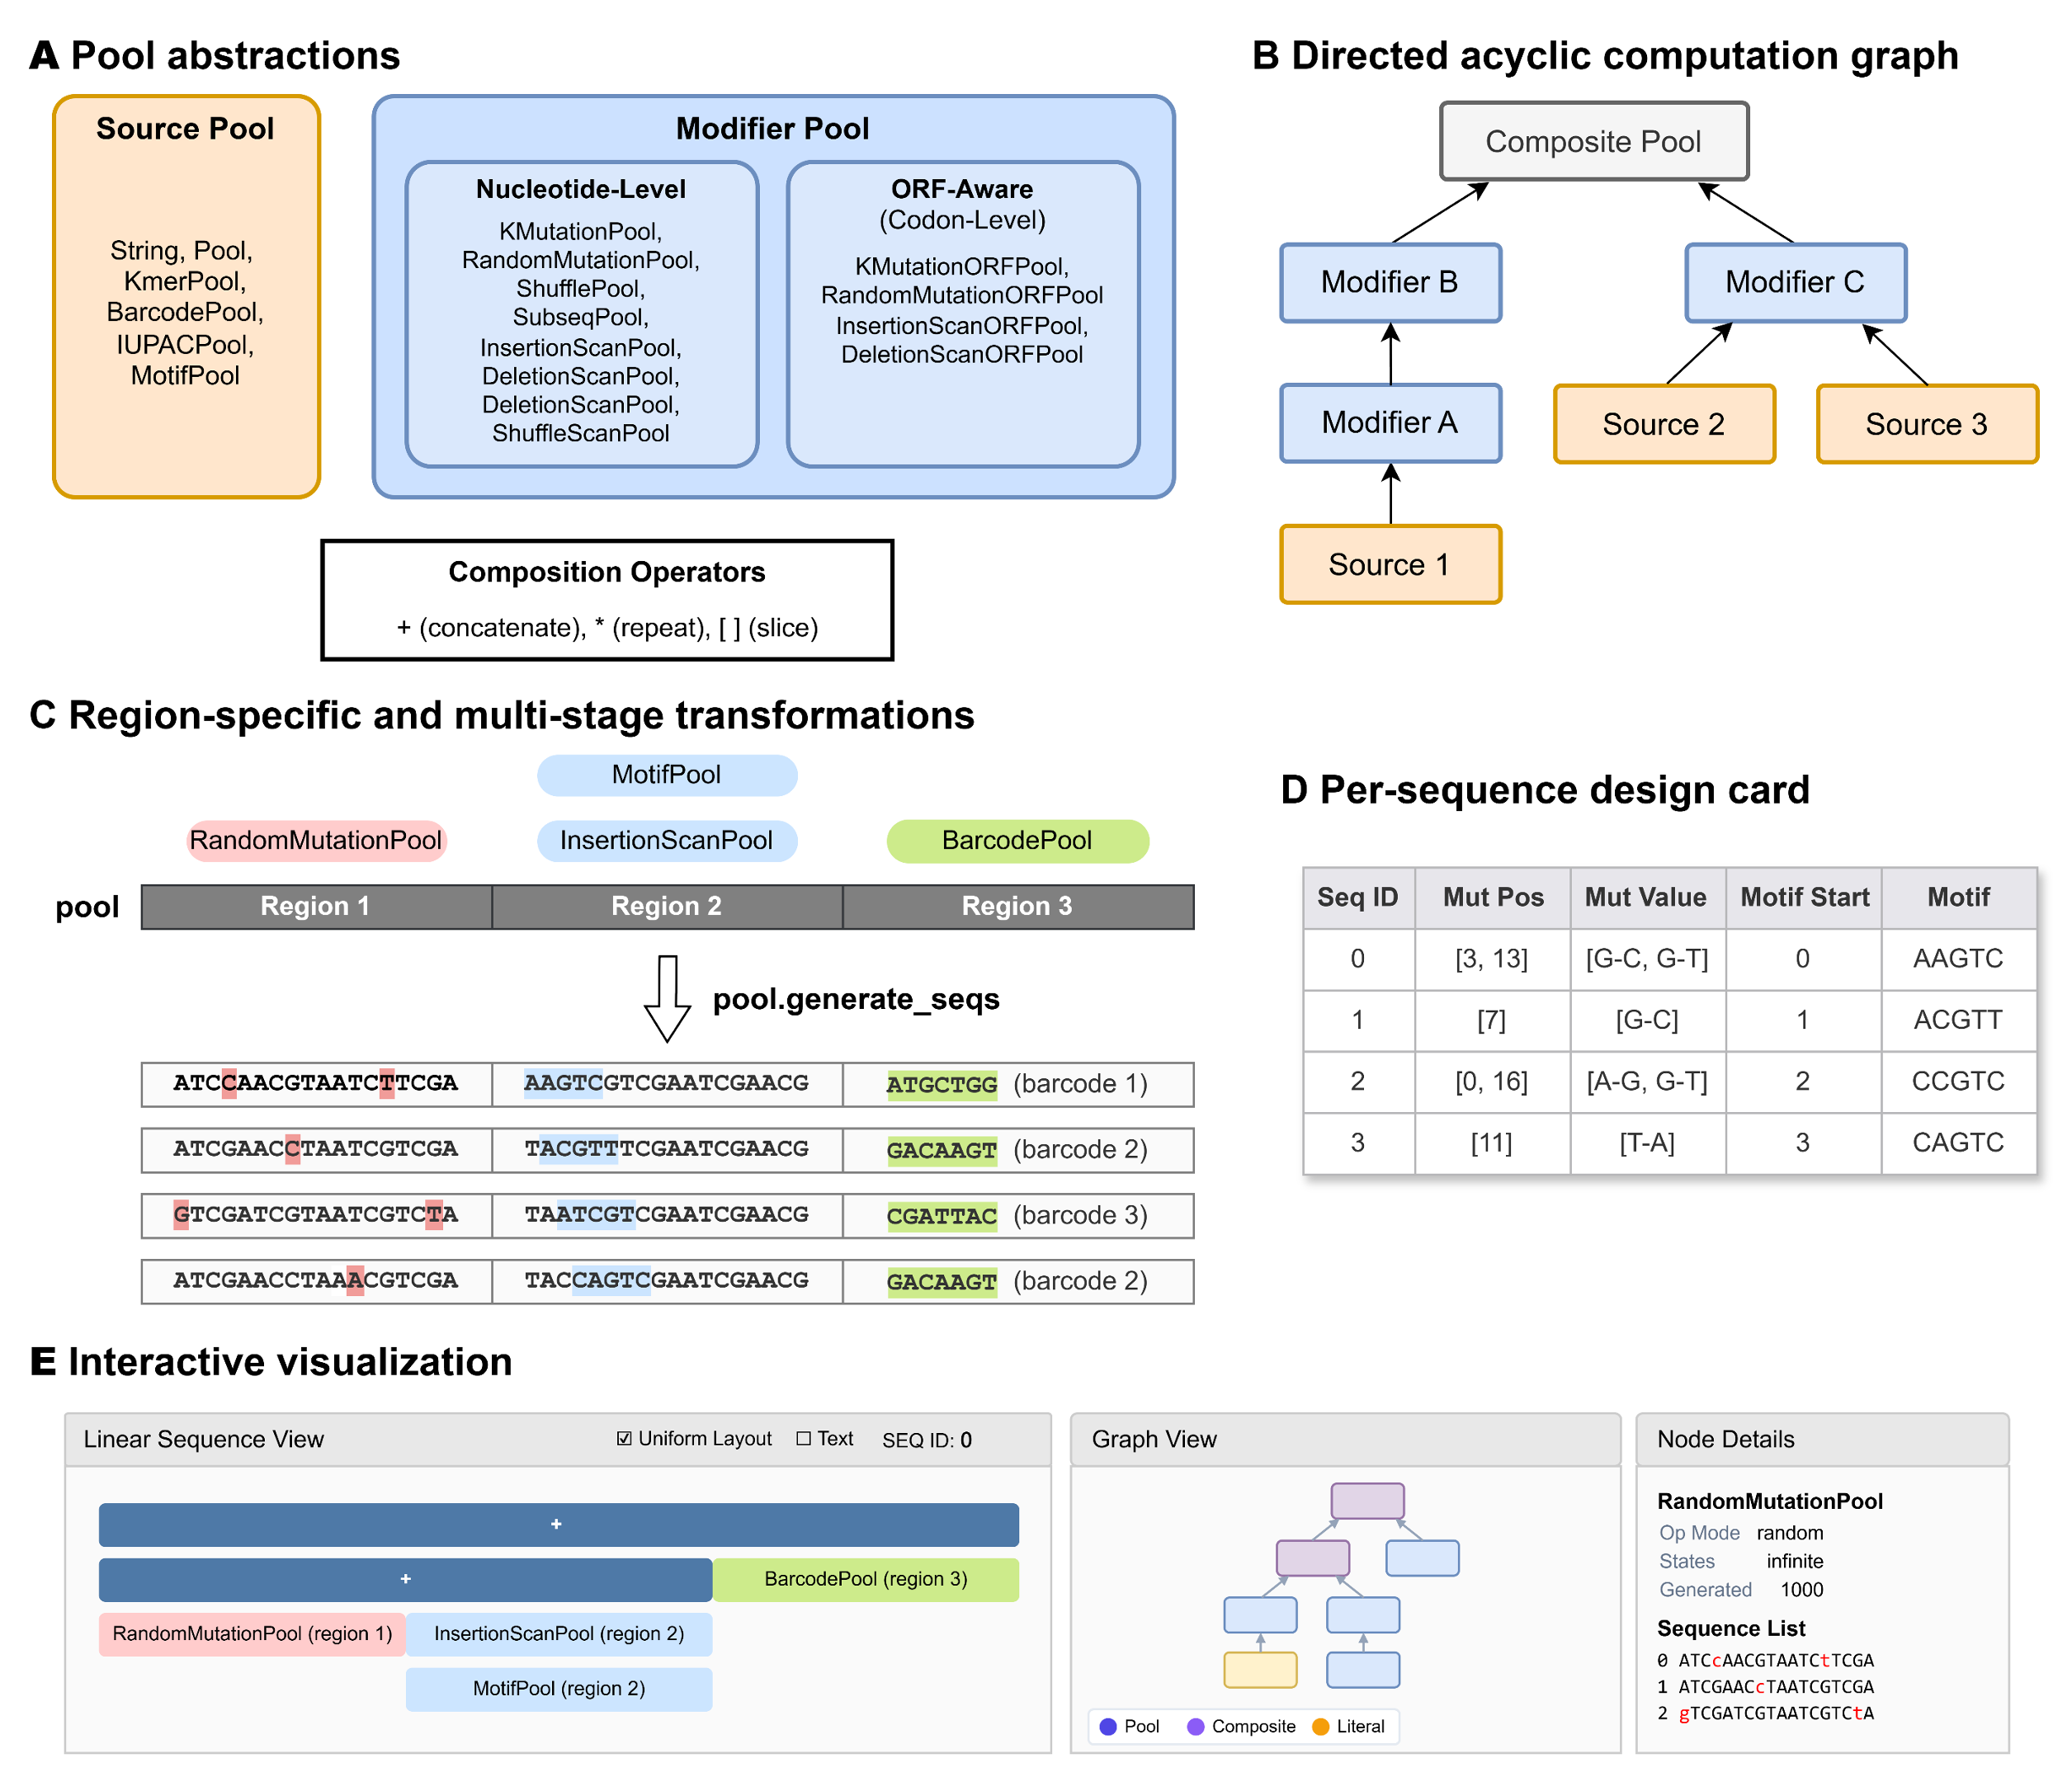
\includegraphics[width=\textwidth]{fig1.png}
\caption{\textbf{Overview of PoolParty architecture and capabilities.} 
\textbf{(A)} Pool abstractions. Source Pools (yellow) generate sequences de novo; Modifier Pools (blue) transform upstream sequences at either the nucleotide level or in an ORF-aware (codon-level) manner. Composition operators (\texttt{+}, \texttt{*}, \texttt{[]}) combine Pools algebraically.
\textbf{(B)} Directed acyclic computation graph. Pools compose into a DAG with source Pools at the leaves, modifier Pools as intermediate nodes, and the composite Pool at the root.
\textbf{(C)} Region-specific and multi-stage transformations. A three-region construct applies different Pool types to each region: RandomMutationPool introduces point mutations in Region 1 (red highlights), InsertionScanPool combined with MotifPool inserts motifs in Region 2, and BarcodePool appends unique barcodes in Region 3 (green). Calling \texttt{pool.generate\_seqs} produces the enumerated library.
\textbf{(D)} Per-sequence design cards. Machine-readable metadata records mutation positions, mutation values, motif insertion sites, and motif sequences for each library member, enabling reproducibility and downstream analysis.
\textbf{(E)} Interactive visualization. The Linear Sequence View displays the stacked regional architecture, the Graph View shows the Pool DAG, and the Node Details panel summarizes Pool parameters and sample sequences.}
\label{fig:overview}
\end{figure*}


\begin{figure*}[t]
    \centering
    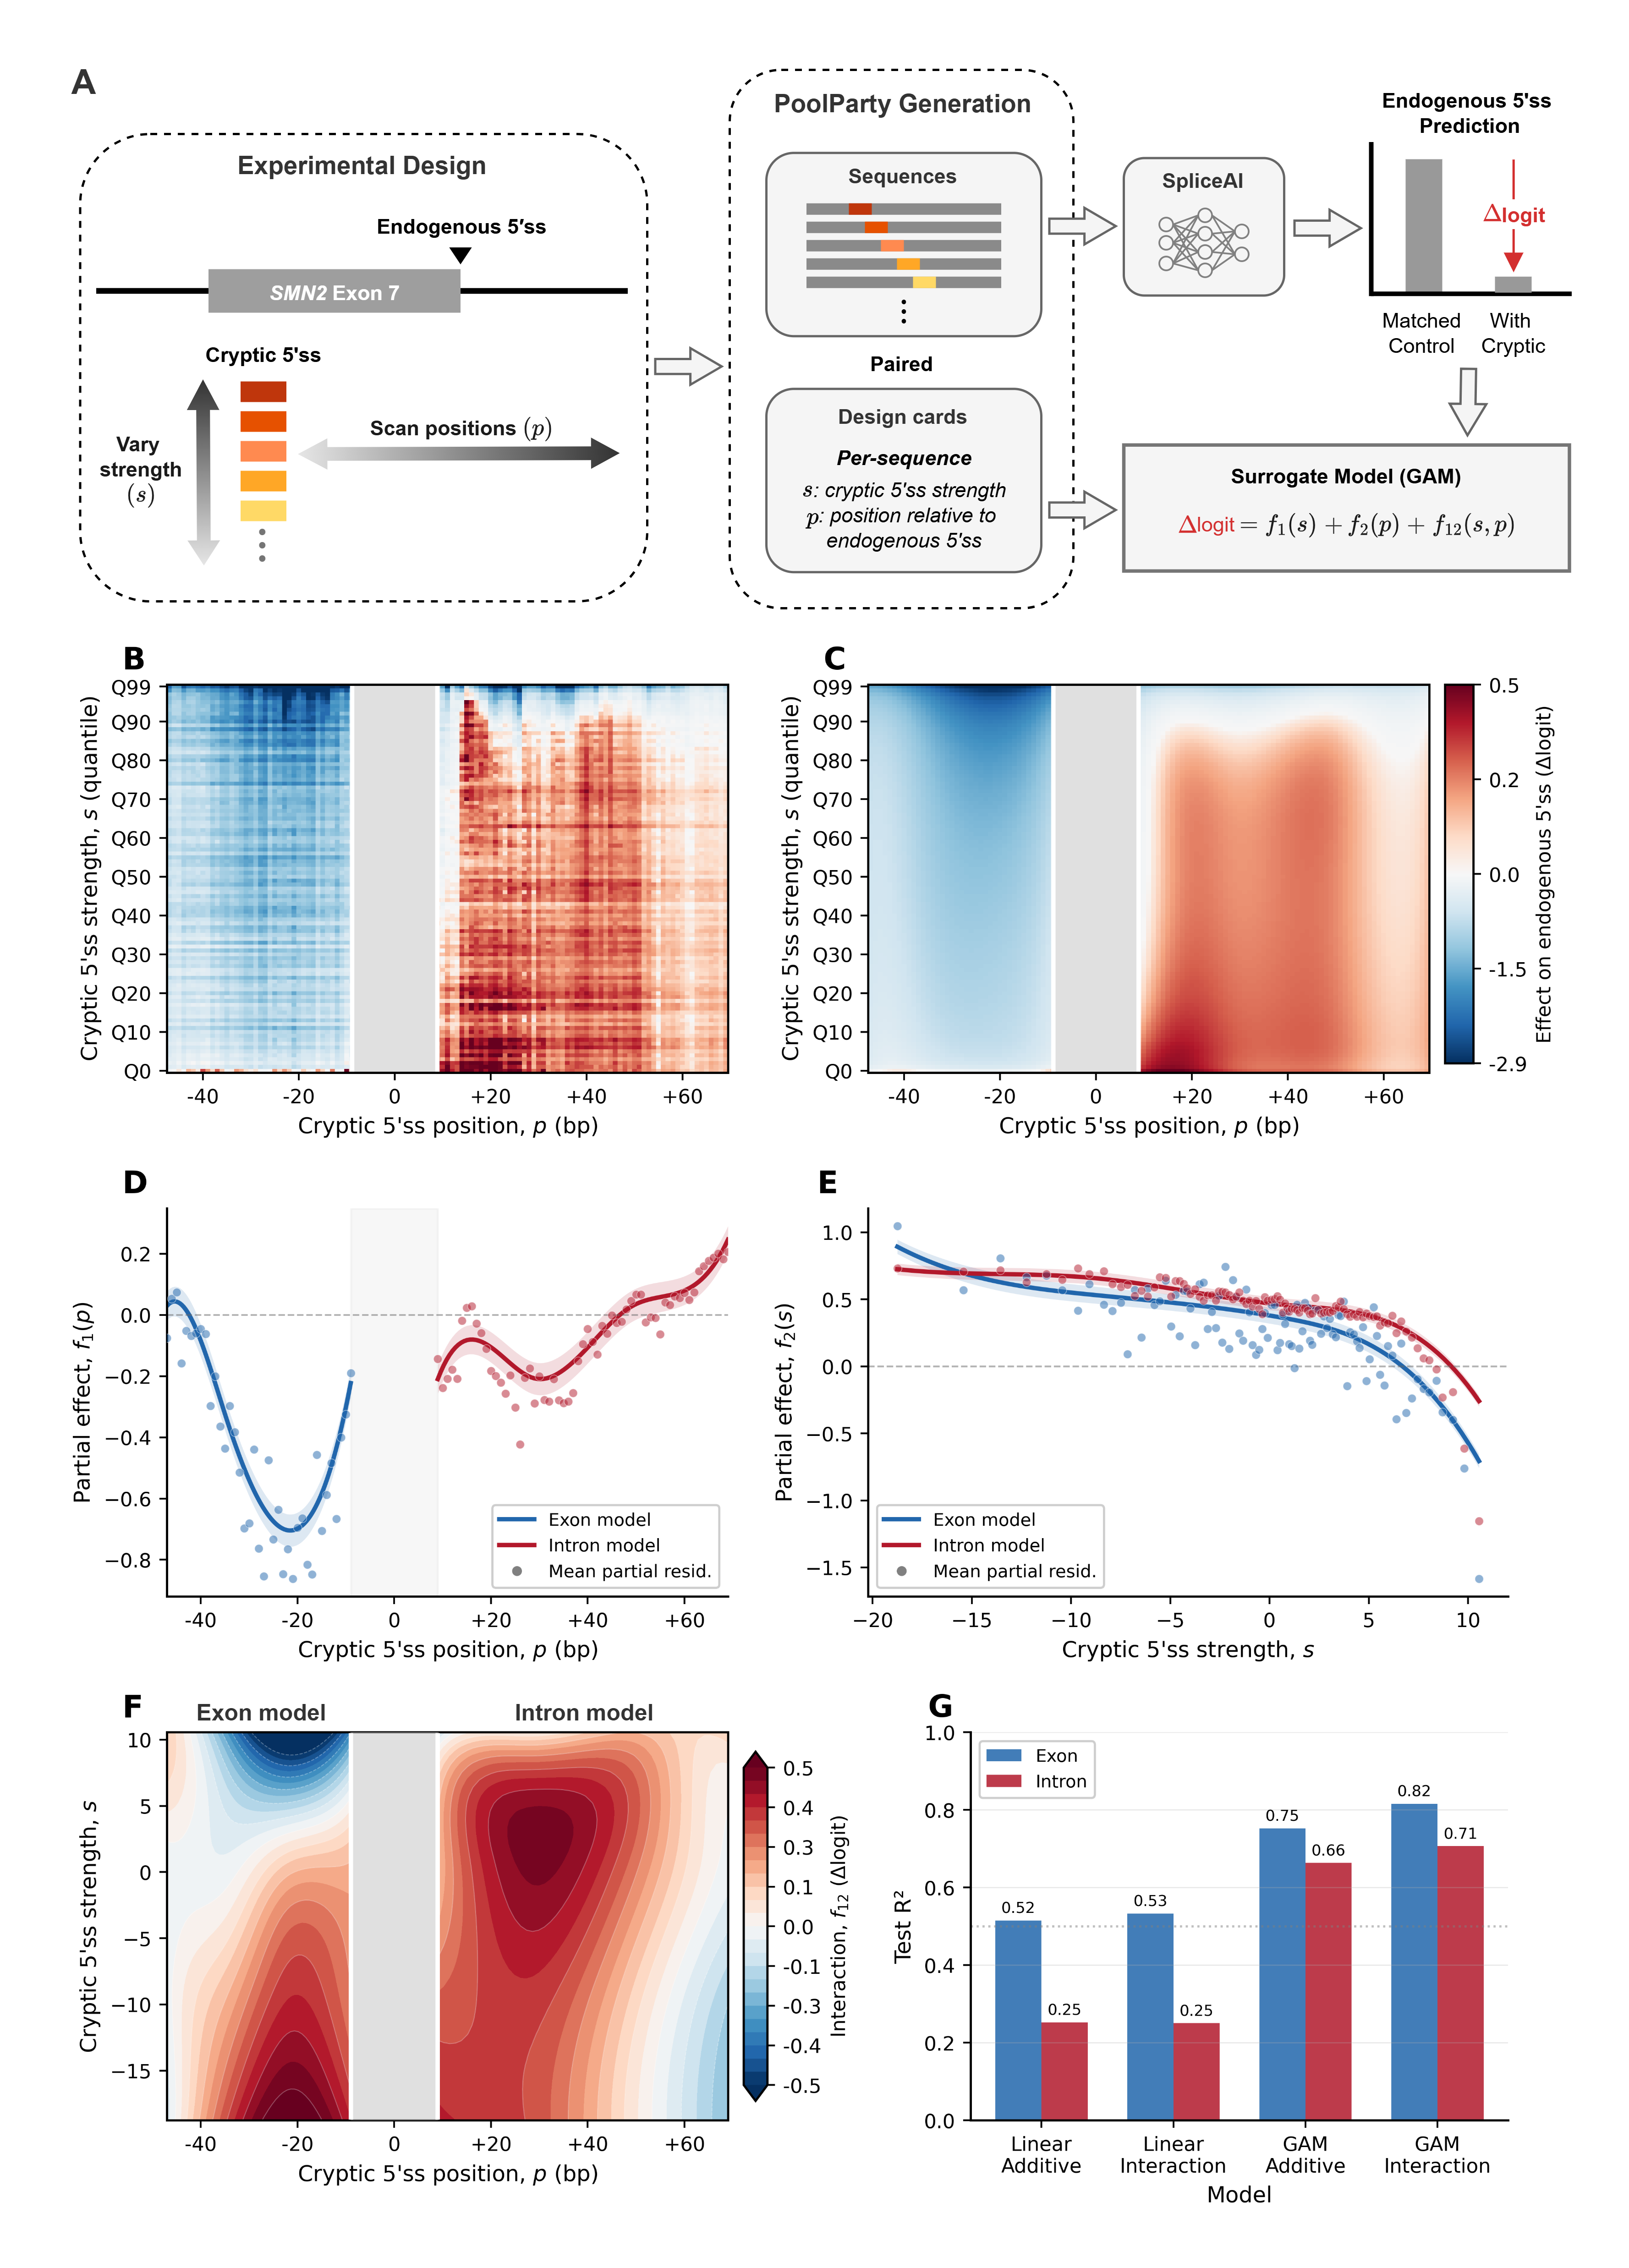
\includegraphics[width=6.5in]{fig3.png}
    \caption{\textbf{Lead sentence} 
    \textbf{(A)} Blots}
    \label{fig:application}
\end{figure*}

\section{Discussion}

PoolParty provides a unified framework for oligonucleotide pool design that addresses a significant gap in the current software landscape. By representing design operations as composable Pool objects that form directed acyclic computation graphs, PoolParty enables researchers to specify complex multi-region, multi-stage library designs declaratively rather than through ad hoc scripting. The automatic generation of per-sequence design cards ensures that every library member carries machine-readable provenance metadata, supporting reproducibility, auditing, and integration with downstream analysis pipelines.

Several aspects of PoolParty's design merit emphasis. First, the separation of sequential and random modes at the per-Pool level allows users to combine exhaustive enumeration (e.g., all single-nucleotide variants in a regulatory element) with stochastic sampling (e.g., random barcodes) within the same library, a flexibility that is difficult to achieve with existing tools. Second, the ORF-aware Pool variants ensure that codon structure and reading frames are preserved when mutating coding sequences, addressing a common source of errors in DMS library design. Third, the interactive visualization tool provides immediate feedback on library architecture, helping users catch design errors before committing to synthesis.

PoolParty does have limitations. The current implementation is optimized for libraries of moderate size (up to millions of sequences) generated on a single machine; very large design spaces may require distributed computation or streaming generation, which are not yet supported. Additionally, PoolParty focuses on sequence generation rather than synthesis optimization; users who require GC content balancing, homopolymer avoidance, or other synthesis constraints should apply post-processing filters or use complementary tools such as DnaChisel \citep{Zulkower2020}.

Looking forward, we envision several extensions. Integration with constraint solvers could enable joint optimization of library coverage and synthesis feasibility. Support for paired-end and long-read sequencing adapters would streamline library preparation workflows. Finally, a web-based interface could make PoolParty accessible to users without Python programming experience.

In summary, PoolParty transforms oligonucleotide pool design from an error-prone, ad hoc process into a structured, transparent, and reproducible workflow. We anticipate that it will accelerate the design and execution of MPRAs, DMS experiments, and other high-throughput functional genomics assays.

\section{Competing interests}
The authors declare no competing interests. 

\section{Author contributions statement}
Z.L concieved the project. J.B.K designed the project, wrote the software, and wrote the manuscript. J.B.K supervised the research. 

\section{Acknowledgments}
This work was supported in part by: NIH grants R01HG011787 (J.B.K, Z.L.). Computational equiptment was supported by NIH grant S10OD028632.

\bibliography{reference}
\end{document}
